\documentclass[border=10pt]{standalone}
\usepackage[svgnames]{xcolor}
\usepackage{amsmath}
\usepackage{pgfplots}
\pgfplotsset{compat=newest}
\usepackage[sfdefault]{FiraSans}
\usepackage{FiraMono}
\renewcommand*\familydefault{\sfdefault}
\begin{document}
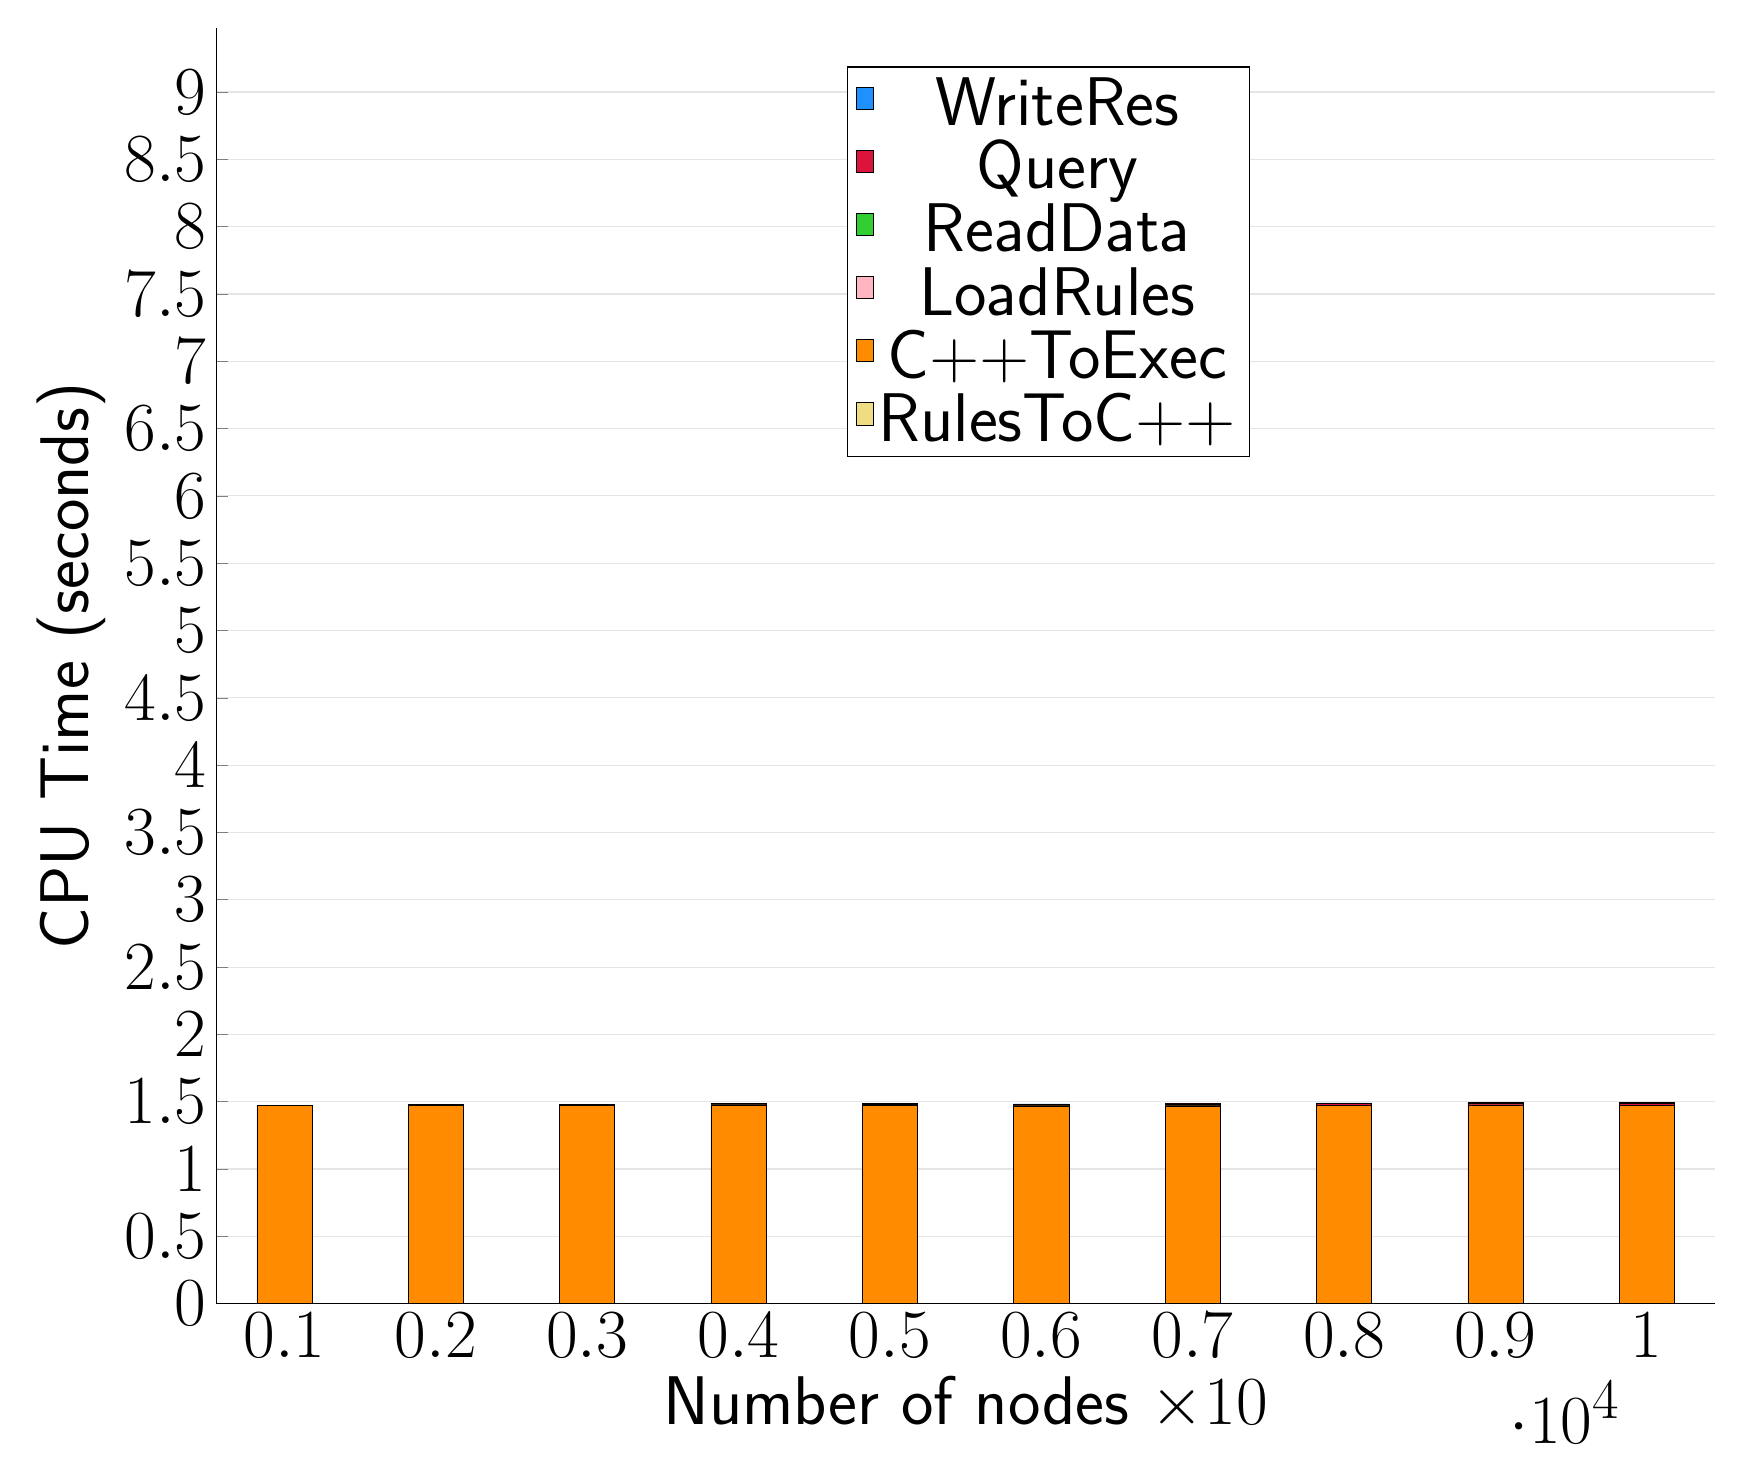
\begin{tikzpicture}
\begin{axis}[
   ybar stacked,
   width=1.7\textwidth,
   bar width=0.7cm,
   ymajorgrids, tick align=inside,
   major grid style={draw=gray!20},
   xtick=data,
   ymin=0, ymax=9.474,
   axis x line*=bottom,
   axis y line*=left,
   enlarge x limits=0.05,
   legend style={
       at={(0.69, 0.97)},
       anchor=north east,
       legend columns=1,
       font=\Huge,
   },
   ylabel={CPU Time (seconds)},
   xlabel={Number of nodes $\times 10$},
   label style={font=\Huge},
   tick label style={font=\Huge},
]
\addlegendimage{fill=DodgerBlue, draw=black, line width=0.2pt}
\addlegendentry{WriteRes}
\addlegendimage{fill=Crimson, draw=black, line width=0.2pt}
\addlegendentry{Query}
\addlegendimage{fill=LimeGreen, draw=black, line width=0.2pt}
\addlegendentry{ReadData}
\addlegendimage{fill=LightPink, draw=black, line width=0.2pt}
\addlegendentry{LoadRules}
\addlegendimage{fill=DarkOrange, draw=black, line width=0.2pt}
\addlegendentry{C++ToExec}
\addlegendimage{fill=LightGoldenrod, draw=black, line width=0.2pt}
\addlegendentry{RulesToC++}
\addplot +[fill=LightGoldenrod, draw=black, line width=0.2pt] coordinates {
(1000, 0.0)
(2000, 0.0)
(3000, 0.0)
(4000, 0.0)
(5000, 0.0)
(6000, 0.0)
(7000, 0.0)
(8000, 0.0)
(9000, 0.004000000000000001)
(10000, 0.0020000000000000005)
};
\addplot +[fill=DarkOrange, draw=black, line width=0.2pt] coordinates {
(1000, 1.4700000000000002)
(2000, 1.472)
(3000, 1.472)
(4000, 1.4760000000000002)
(5000, 1.47)
(6000, 1.468)
(7000, 1.4679999999999997)
(8000, 1.47)
(9000, 1.468)
(10000, 1.4679999999999997)
};
\addplot +[fill=LightPink, draw=black, line width=0.2pt] coordinates {
(1000, 0.00016639999999999998)
(2000, 0.0001746)
(3000, 0.0001682)
(4000, 0.0001662)
(5000, 0.0001818)
(6000, 0.0001728)
(7000, 0.0001706)
(8000, 0.00018360000000000002)
(9000, 0.0001744)
(10000, 0.0001694)
};
\addplot +[fill=LimeGreen, draw=black, line width=0.2pt] coordinates {
(1000, 0.0008546)
(2000, 0.001211)
(3000, 0.0016538)
(4000, 0.0020718)
(5000, 0.002424)
(6000, 0.0027264000000000004)
(7000, 0.0030444)
(8000, 0.0035477999999999994)
(9000, 0.0033313999999999996)
(10000, 0.0041838)
};
\addplot +[fill=Crimson, draw=black, line width=0.2pt] coordinates {
(1000, 0.0022238)
(2000, 0.0039704)
(3000, 0.00598)
(4000, 0.00779)
(5000, 0.009280199999999999)
(6000, 0.0097022)
(7000, 0.011700799999999999)
(8000, 0.0138316)
(9000, 0.01305)
(10000, 0.015516600000000002)
};
\addplot +[fill=DodgerBlue, draw=black, line width=0.2pt] coordinates {
(1000, 0.001306)
(2000, 0.0016687999999999998)
(3000, 0.0018242000000000002)
(4000, 0.0017274)
(5000, 0.0026190000000000002)
(6000, 0.0033908000000000002)
(7000, 0.003269)
(8000, 0.0038314)
(9000, 0.0038378)
(10000, 0.0044506)
};
\end{axis}
\end{tikzpicture}

\end{document}
